\documentclass[11pt]{article}
\usepackage[utf8]{inputenc}
\usepackage[T1]{fontenc}
\usepackage{amsmath}
\usepackage{amsfonts}
\usepackage{amssymb}
\usepackage[version=4]{mhchem}
\usepackage{stmaryrd}
\usepackage{graphicx}
\usepackage[export]{adjustbox}
\graphicspath{ {./images/} }
\usepackage{hyperref}
\hypersetup{colorlinks=true, linkcolor=blue, filecolor=magenta, urlcolor=cyan,}
\urlstyle{same}

\title{Reading }

\author{}
\date{}


\begin{document}
\maketitle
Distinguishing Hedge Funds

The term hedge fund originated with the first hedge fund, A.W. Jones \& Co., which was established in 1949 and invested in both long and short equity positions. The intent was to limit market risk while focusing on stock selection. This hedge fund operated in relative obscurity until an article published in Fortune magazine in April 1966 spotlighted Alfred Winslow Jones. ${ }^{1}$ Carol Loomis (April 1966), The Jones Nobody Keeps Up With, Fortune, 237-47. The interest in Jones's product was large, and within two years, a survey conducted by the SEC established that the number of hedge funds had grown from 1 to 140. Many hedge funds were liquidated during the bear market of the early 1970s, and the hedge fund industry did not regain popularity until the end of the 1980s. The appeal of hedge funds increased tremendously in the 1990s, and by 2021, there were around 9,300 hedge funds with more than $\$ 4$ trillion in total assets. For comparison, the amount of total assets for mutual funds and exchange-traded funds (ETFs) was $\$ 30$ trillion in 2021.

The term hedge fund has evolved and expanded to include funds that do not necessarily hold hedged positions. In this course, hedge funds are distinguished from their traditional counterpart, mutual funds, with the definition in the next section.

\section*{Three Primary Elements of Hedge Funds}
A hedge fund is an investment pool or investment vehicle that (1) is privately organized in most jurisdictions; (2) usually offers performance-based fees to its managers; and (3) can usually apply leverage, invest in private securities, invest in real assets, actively trade derivative instruments, establish short positions, invest in structured products, and generally hold relatively concentrated positions.

First, hedge funds are privately organized and generally unlisted. They are designed in this way to pool the resources of sophisticated investors and provide opportunities that are not available through traditional, regulated pools or that are more easily or cost effectively executed using private vehicles. Hedge funds are typically less regulated than public investment vehicles because of their privately organized nature. (In some jurisdictions, the fund management company of a hedge fund has to be registered in the same manner as the fund management company of a mutual fund.)

Hedge funds are designed to be private by using one or more safe harbor provisions. In investments, a safe harbor denotes an area that is explicitly protected by one set of regulations from another set of regulations. In the United States, for example, hedge funds are specifically exempt from the disclosure requirements of the U.S. Investment Company Act of 1940 through one of two exemptions, or safe harbors, available to funds that are not advertised or offered to the general public.

Second, hedge funds typically offer incentive-based fees to attract and motivate top managers. These fees are designed to align the interests of the managers with the investors, as is detailed in a subsequent section of this session. The potentially high and performance-based compensation to managers is central to the idea that hedge fund management implements highly sophisticated investment strategies that offer investment opportunities distinct from those available in the public investment space. How managers are compensated can change the nature of an investment, including its risks and returns.

Third, hedge funds typically allow one or more aspects of greater investment flexibility than do traditional investment vehicles. This investment flexibility is detailed in the next section.

\section*{Six Investment Flexibilities of Hedge Funds}
The six major investment flexibilities used by hedge funds are:

\begin{enumerate}
  \item Hedge fund strategies often invest in nonpublic, unlisted securities-that is, securities that have been issued to investors without the support of a prospectus and a public offering and that are not publicly traded.

  \item Hedge funds often use leverage, at times very large amounts. Mutual funds in the United States are limited in the amount of leverage they can employ, able to borrow up to $33 \%$ of their net asset base. Hedge funds do not have this restriction. Consequently, it is not unusual to see some hedge fund strategies employing leverage up to 10 times their net asset base.

  \item Hedge funds often use derivative strategies much more predominantly than do traditional investment vehicles such as mutual funds. In some strategies, such as convertible arbitrage or managed futures, the ability to sell or buy options or futures is a key component of executing the fund's strategy. The use of derivative strategies may result in nonlinear cash flows that may require more sophisticated risk management techniques. Derivative strategies can also increase fund leverage.

  \item Hedge funds take short positions in securities to increase return or reduce risk. The ability to take very large short positions in public securities is one of the key distinctions between hedge fund managers and traditional money managers. Hedge fund managers explicitly incorporate their ability to short sell securities into their investment strategies. For example, equity long/short hedge funds tend to buy and short sell securities within the same industry to maximize their return but also to control their risk. This is very different from the actions of most traditional money managers, who are tied to a long-only securities benchmark. Shorting can also have the effect of increasing fund leverage.

  \item Hedge funds sometimes trade in more esoteric or riskier underlying investments, such as those that are structured.

  \item Hedge funds tend to be more actively managed than traditional investment vehicles, with more complex strategies and with more dynamic risk exposures than traditional funds, which are often constrained to generating performance that is linked to a benchmark.

\end{enumerate}

Some funds are considered hedge funds even though they possess only one or two of the characteristics discussed in this section. Hedge funds are not defined by sharp lines of division from other investments; in fact, as alternative investments evolve, it is becoming increasingly difficult to distinguish hedge funds from other alternative investment vehicles, such as private equity funds.

The side-by-side comparison of mutual funds and hedge funds in the below exhibit summarizes distinctions between mutual funds and hedge funds commonly observed in various jurisdictions throughout the world.

\begin{center}
\begin{tabular}{|lll|}
\hline
 & Mutual Funds & Hedge Funds \\
\hline
Offering method (documentation) & Prescribed, detailed & Flexible, voluntary \\
Disclosure requirements & Prescribed, detailed & Flexible, voluntary \\
Investment strategies available & Restricted & Unrestricted \\
Concentration limits & Restricted & Unrestricted \\
Use of leverage & Restricted & Unrestricted \\
Use of derivatives & Restricted & Unrestricted \\
Allowable investors & Unrestricted (anyone) & Restricted (accredited only) \\
Manager registration & Required & Required \\
\hline
\end{tabular}
\end{center}

The greater restrictions on mutual funds facilitate the distribution of shares more broadly to the public, whereas the lesser restrictions on hedge funds are consistent with limited distribution to the accredited investors or qualified purchasers whom regulators deem able to properly evaluate the risks inherent in the offering.

There are many reasons for the huge interest in hedge funds. First, hedge fund returns can offer low correlation with traditional investments and therefore serve as diversifiers. Strong bear markets over the past 25 years have fueled the interest of those investors who saw their traditional stock portfolios decline in value. Second, many investors recognize the advantage that hedge funds have with regard to investment flexibility, such as being able to go both long and short to maximize the value of their information about stocks, bonds, and other securities. Third, many investors sought the potential double-digit returns of the hedge fund industry, especially when other investment opportunities, such as bonds, offered low or even negative returns after taxes and anticipated inflation.

While hedge funds enjoyed enormous growth prior to 2007, the industry saw a decline in both the assets and the number of funds after 2007. The financial crises that began in 2007 caused the hedge fund industry to post negative returns and experience the first asset net outflows since 1994. Between the end of 2007 and the end of 2009, Hedge Fund Research, Inc. (HFR), a major firm specializing in the indexation and analysis of hedge funds, estimates that hedge fund industry assets declined by $25 \%$, as fund losses totaled $\$ 176$ billion and investors withdrew an additional $\$ 285$ billion.

The following exhibit, Estimated Number of Funds Launched/Liquidated, shows the change in the number of hedge funds over time. Notice that the hedge fund industry added new funds each year from 1996 to 2007. After significant net attrition in 2008 and 2009, the number of hedge funds continued to grow through 2014, as more funds were launched than liquidated. More recently, we've witnessed net attrition from 2015 through 2020, as performance has been challenging and asset flows have experienced more volatility.

\begin{center}
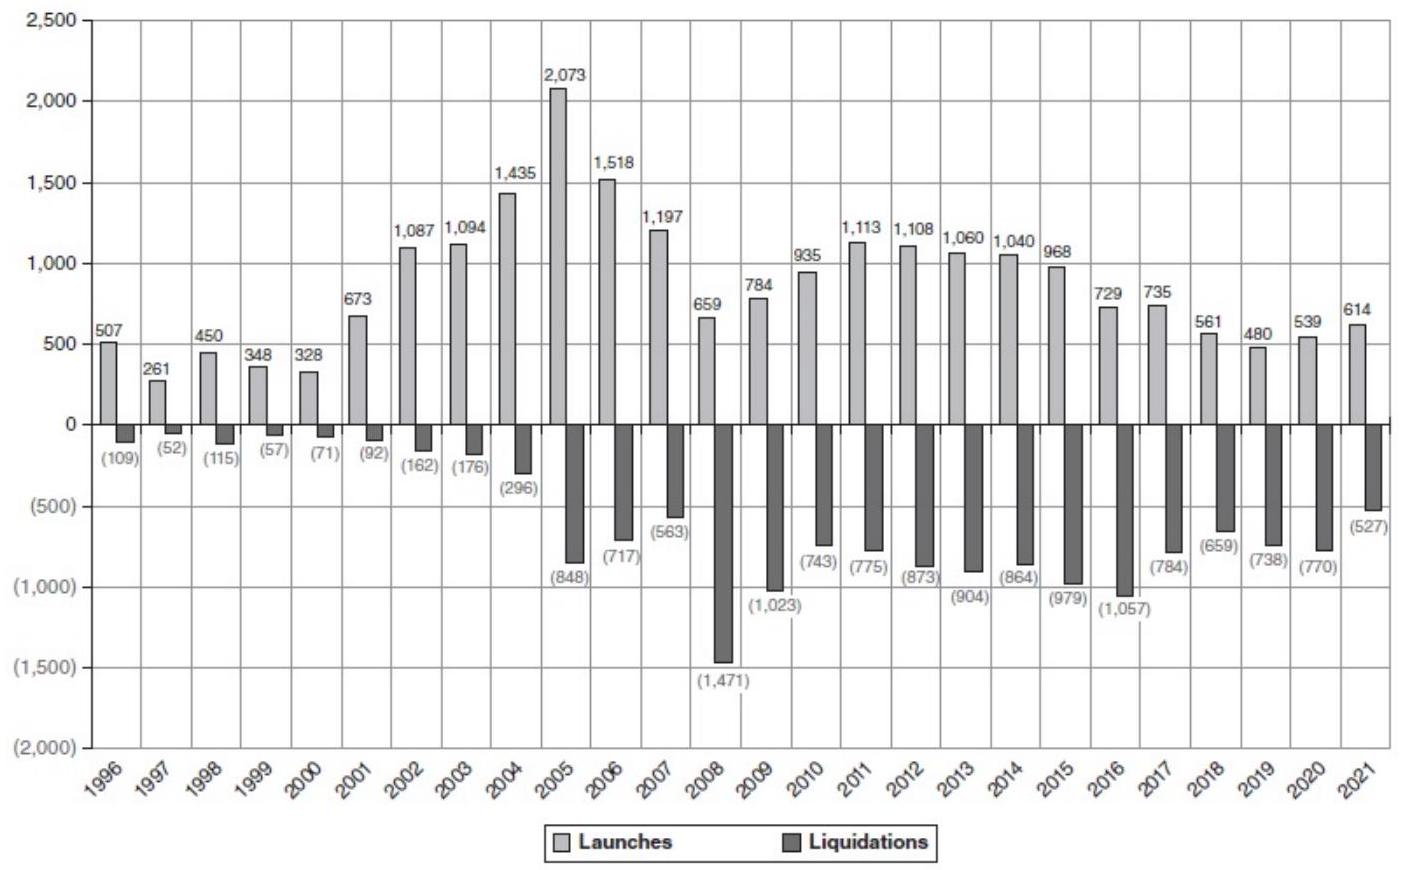
\includegraphics[max width=\textwidth]{2024_04_09_501764bcdced134762e2g-2}
\end{center}

Estimated Number of Funds Launched/Liquidated

Source: Data from HFR Industry Reports, HFR, Inc. @) 2021, \href{http://www.hedgefundresearch.com}{www.hedgefundresearch.com}.

\section*{Industry Concentration}
The year 2008 was an especially difficult year for hedge fund investing, with several prominent hedge fund frauds and massive fund liquidations. These events served to accelerate the trend of consolidation within the hedge fund industry. Consolidation is an increase in the proportion of a market represented by a relatively small number of participants (i.e., the industry concentration). While there were more than 9,300 hedge funds and funds of funds at the end of 2021 , institutional investors are showing a clear preference for the largest funds. An explanation is that hedge fund investors are seeking to invest with stable firms with demonstrated risk management processes and strong operational risk controls. Simply put, large funds are perceived as being less risky.

Another reason for hedge fund industry consolidation is the expense to hedge funds of facilitating due diligence by investors. Due diligence processes, discussed in Level II of the CAIA program, are performed by prospective investors prior to consummating their investment in a hedge fund. These due diligence processes place a substantial burden on the managers of hedge funds targeted for investment. The largest hedge funds can best afford the investments in staff and systems required to pass the strict investigations made by today's post-crisis institutional investors.

The next exhibit, Distribution of Industry Assets by Firm AUM Tier, shows the consolidation in the hedge fund industry, as the largest funds continue to grow as a percentage of industry assets. Approximately $15 \%$ of hedge fund management firms manage more than $\$ 500$ million. Combined, these funds manage $90 \%$ of all industry assets. These large funds may be successful at raising assets because they have made large investments in compliance and risk management infrastructures necessary to pass the enhanced due diligence processes of large institutional investors. This leaves nearly 8,000 hedge funds competing for $10 \%$ of industry assets under management (AUM).

\begin{center}
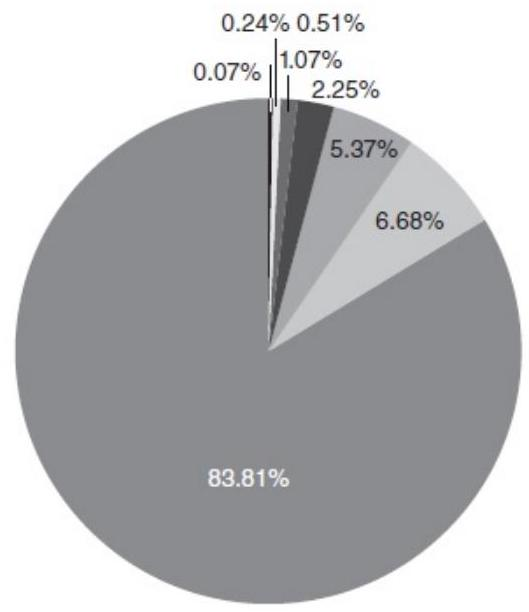
\includegraphics[max width=\textwidth]{2024_04_09_501764bcdced134762e2g-3}
\end{center}

Distribution of Industry Assets by Firm AUM Tier

Source: Data from HFR Industry Reports, HFR, Inc. @ 2021, \href{http://www.hedgefundresearch.com}{www.hedgefundresearch.com}.

NOTE

\begin{enumerate}
  \item Carol Loomis (April 1966), The Jones Nobody Keeps Up With, Fortune, 237-47.
\end{enumerate}

\end{document}